\makeatletter
\def\@makechapterhead#1{%
  \vspace*{10\p@}%
  {\parindent \z@ \raggedleft \normalfont
    \ifnum \c@secnumdepth >\m@ne
      \if@mainmatter
        \LARGE\bfseries \@chapapp\space \thechapter
	\vskip 4pt
        \hrule height 2pt
        \par\nobreak
        \vskip 5\p@
      \fi
    \fi
    \interlinepenalty\@M
    \huge \bfseries #1\par\nobreak
\vskip 5pt

\hrule height 2pt   
 \vskip 10\p@  
  }}
\makeatother

\chapter{BJT Biasing}\label{chap3}
\addtocontents{toc}{\protect\contentsline{chapter}{\protect Chapter \numberline{\thechapter.}
  BJT Biasing}{\thepage--\pageref{3end}}}  

\medskip
\section{Operating Point}\label{sec3.1}

In order for a transistor to amplify, it has to be properly biased. That means, we have to set a fixed value of certain currents and voltages in the transistor used. These values of currents and voltages corresponds to a point on the transistor's output characteristics at which it operates. This point is called operating point or quiescent point or Q-point. Consider the circuit shown below in Figure.
\begin{figure}[H]
\centering
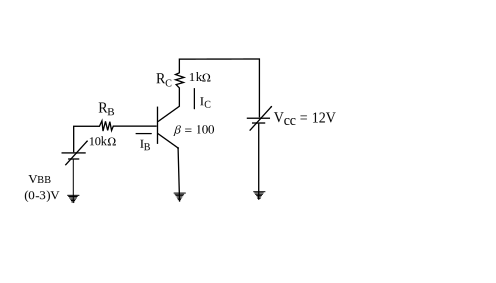
\includegraphics{chap3/fig3.1.eps}
\end{figure}

Here the transistor is biased with two variable dc power supplies namely $\rmV_{\rmB\rmB}$ and $\rmV_{\rmC\rmC}$ to obtain the fixed values of base current $\rmI_{\rmB}$, collector current $\rmI_{\rmC}$ and collector-to-emitter voltage $\rmV_{\rmC\rmE}$. The output characteristics of the transistor is shown in Fig. below. We will use these characteristics to graphically illustrate the effects of dc bias.

Consider that $\rmV_{\rmB\rmB}$ is adjusted to produce a base current $\rmI_{\rmB}=50\mu\rmA$. Since $\rmI_{\rmC}=\beta \rmI_{\rmB}$, the collector current is $\rmI_{\rmC}=100\times 50\mu = 5\text{~mA}$. Then $\rmV_{\rmC\rmE}=\rmV_{\rmC\rmC}-\rmI_{\rmC}\rmR_{\rmC}=12-(5\rmm)(1\rmk)=7\rmV$. This Q-point is shown in Fig. as $\rmQ_{1}$.

Next, consider that $\rmV_{\rmB\rmB}$ is increased to produce $\rmI_{\rmB}=75\mu\rmA$. Then $\rmI_{\rmC}=\beta\rmI_{\rmB}=100\times 75\mu=7.5\text{~mA}$ and $\rmV_{\text{CE}}=12-(7.5\rmm)(1\rmk)=4.5\rmV$. This Q-point is shown in Fig. as $\rmQ_{2}$. 

Finally, consider that $\rmV_{\rmB\rmB}$ is increased to produce $\rmI_{\rmB}=100\mu\rmA$. Then $\rmI_{\rmC}=\beta\rmI_{\rmB}=100\times 100\mu=10\text{~mA}$ and $\rmV_{\text{CE}}=12-(10\rmm)(1\rmk)=2\rmV$. This Q-point is shown in Fig. as $\rmQ_{3}$.
\begin{figure}[H]
\centering
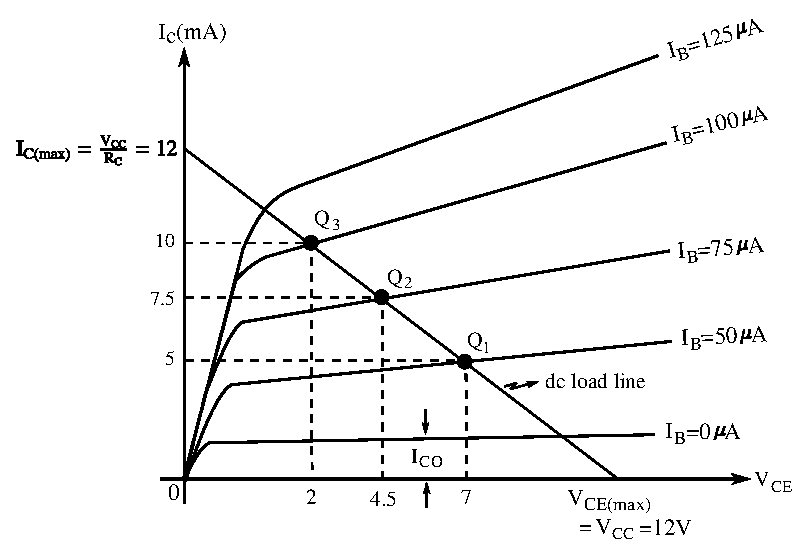
\includegraphics[scale=.9]{chap3/fig3.2.eps}
\end{figure}

It is noticed that, when $\rmI_{\rmB}$ increases, $\rmI_{\rmC}$ increases and $\rmV_{\rmC\rmE}$ decreases. Thus as $\rmV_{\rmB\rmB}$ is varied up or down, the dc operator point (Q-point) of the transistor moves along a straight line called `dc load line'.

The dc load line intersects the $\rmV_{\text{CE}}$ axis at 12V, the point where $\rmV_{\text{CE}}\simeq \rmV_{\text{CC}}$. This is transistor's cut-off point because $\rmI_{\rmB}$ and $\rmI_{\rmC}$ are zero (ideally). Actually, there is a small leakage current $\rmI_{\text{CO}}$ as shown and $\rmV_{\text{CE}}$ is slightly less than 12V. But the small difference can be neglected. The dc load line interested $\rmI_{\rmC}$ axis at 12mA ideally. This is transistor's saturation point because $\rmI_{\rmC}$ is maximum at this point where $\rmV_{\text{CE}}=0\rmV$ and $\rmI_{\rmC}=\dfrac{\rmV_{\text{CC}}}{\rmR_{\rmC}}$. Actually, there is a small voltage $\rmV_{\text{CE(sat)}}$ across the transistor and $\rmI_{\rmC\text{(sat)}}$ is slightly less than 12\,mA.

Applying KVL to collector loop, we get
\begin{align}
& \rmV_{\text{CC}} = \rmI_{\rmC}\rmR_{\rmC}+\rmV_{\text{CE}}\notag\\[3pt]
& \rmI_{\rmC}=-\left(\frac{1}{\rmR_{\rmC}}\right)\rmV_{\text{CE}}+\frac{\rmV_{\text{CC}}}{\rmR_{\rmC}}\label{eq3.1}
\end{align}

Eqn.~\eqref{eq3.1} corresponds to straight line which slope of $-\dfrac{1}{\rmR_{\rmC}}$ and inter????? and, the cut-off region is called active region of the transistor operation. As long as the transistor is operated in this region, the output voltage is almost a linear reproduction of the input. Generally, the transistor amplifier circuit is designed such that the Q point $\rmV_{\text{CE}_{\rmQ}}$ is almost equal to $\dfrac{1}{2}\rmV_{\text{CC}}$.

The circuit which is designed to operate the transistor in its active region is called `biasing' circuit.

\heading{Biasing Circuits~:}
The different transistor biasing circuits explained are,
\begin{itemize}
\item[(i)] Fixed bias circuit

\item Emitter, stabilized bias circuit

\item Collector feedback bias circuit

\item Voltage divider bias circuit
\end{itemize}

\heading{(i)~ Fixed Bias Circuit~:} (Base Bias Circuit)

Fig. shows a transistor amplifier employing fixed bias.
\begin{figure}[H]
\centering
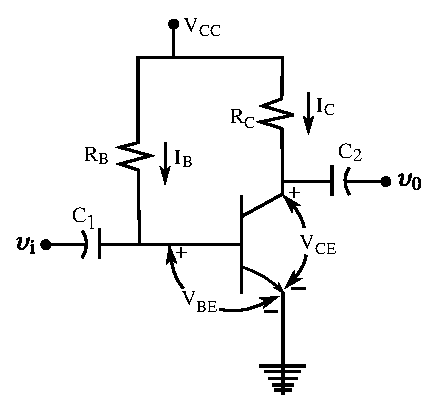
\includegraphics{chap3/fig3.3.eps}
\end{figure}

The dc equivalent circuit is shown below. All capacitors are replaced by open circuit.


Applying KVL to the input side.
\begin{align*}
\rmV_{\text{CC}} &= \rmI_{\rmB}\rmR_{\rmB}+\rmV_{\text{BE}}\\[4pt]
\therefore\quad \rmI_{\rmB} &= \frac{\rmV_{\text{CC}}-\rmV_{\text{BE}}}{\rmR_{\rmB}}\simeq \dfrac{\rmV_{\text{CC}}}{\rmR_{\rmB}}\qquad [\because \ \rmV_{\text{CC}}\gg \rmV_{\text{BE}}]\\[4pt]
\rmI_{\rmC} &= \rmB\rmI_{\rmB} = \beta \left[\frac{\rmV_{\text{CC}}-\rmV_{\text{BE}}}{\rmR_{\rmB}}\right]
\end{align*}
\begin{figure}[H]
\centering
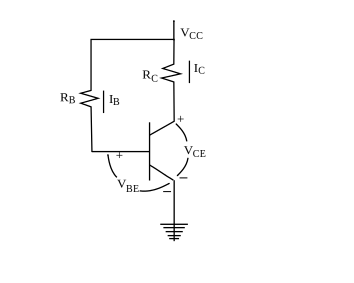
\includegraphics{chap3/fig3.4.eps}
\end{figure}


Since $\rmI_{\rmB}$ is constant for given value of $\rmR_{\rmB}$, the circuit is called fixed bias circuit.

Applying KVL to the output side,
\begin{align*}
\rmV_{\text{CC}} &= \rmI_{\rmC}\rmR_{\rmC}+\rmV_{\text{CE}}\\[4pt]
\rmV_{\text{CE}} &= \rmV_{\text{CC}}-\rmI_{\rmC}\rmR_{\rmC}\\[4pt]
\text{and}\qquad \rmV_{\text{CE}} &= \rmV_{\rmC}-\rmV_{\rmE}=\rmV_{\rmC}
\end{align*}
where $\rmV_{\rmC}$ and $\rmV_{\rmE}$ are the voltages from collector and emitter to ground (reference point) respectively. In this case $\rmV_{\rmE}=0$.

Similarly\qquad $\rmV_{\text{BE}}=\rmV_{\rmB}-\rmV_{\rmE}=\rmV_{\rmB}$.

\begin{center}
\rule{4cm}{1pt}\\
{\bf\Large Problems}\\[-3pt]
\rule{4cm}{1pt}
\end{center}

\begin{problem}\label{prop3.1}
Determine the following for the fixed bias configuration shown below.
\begin{itemize}
\item[(a)] $\rmI_{\rmB_{\rmQ}}$\quad (b)~ $\rmI_{\rmC_{\rmQ}}$\quad (c)~ $\rmV_{\text{CE}_{\rmQ}}$\quad (d)~ $\rmV_{\rmB}$\quad (e)~ $\rmV_{\rmC}$\quad (f)~ $\rmV_{\text{BC}}$~ :~ Given $\rmV_{\text{BE}}$.
\begin{figure}[H]
\centering
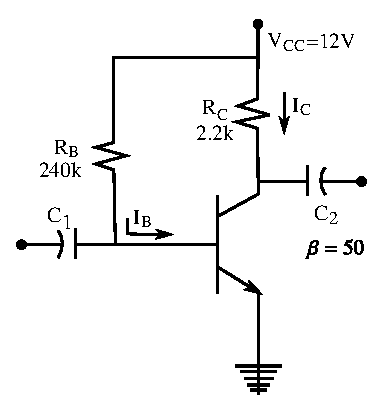
\includegraphics[scale=.95]{chap3/fig3.5.eps}
\end{figure}
\begin{figure}[H]
\centering
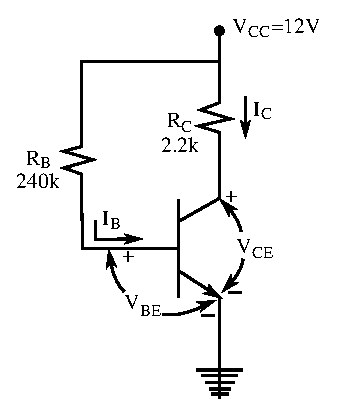
\includegraphics[scale=.95]{chap3/fig3.6.eps}
\end{figure}
\item[(a)] $\rmI_{\rmB_{\rmQ}}=\dfrac{\rmV_{\text{CC}}-\rmV_{\text{BE}}}{\rmR_{\rmB}}=\dfrac{12-0.7}{240\times 10^{3}}=47.05\mu\rmA$

\item[(b)] $\rmI_{\rmC_{\rmQ}}=\beta \rmI_{\rmB_{\rmQ}}=50\times 47.08\times 10^{-6}=2.35\text{~mA}$

\item[(c)] $\rmV_{\text{CE}_{\rmQ}}=\rmV_{\text{CC}}-\rmI_{\rmC_{\rmQ}}\cdot \rmR_{\rmC}=12-(2.35\times 10^{-3})(2.2\times 10^{3})=6.83\rmV$

\item[(d)] $\rmV_{\rmB}=\rmV_{\text{BE}}=0.7\rmV$

\item[(e)] $\rmV_{\rmC}=\rmV_{\text{CE}}=6.83\rmV$

\item[(f)] $\rmV_{\text{BC}}=\rmV_{\rmB}-\rmV_{\rmC}=0.7-6.83=-6.13\rmV$
\end{itemize}
The negative value of $\rmV_{\text{BC}}$ indicates that collector-base junction is reverse biased.
\end{problem}

\vfill\eject

\begin{solution}
$\beta=80$, \ $\rmI_{\rmB}=40\mu\rmA$, \ $\rmV_{\text{BE}}=0.7\rmV$, \ $\rmV_{\text{CC}}=12\rmV$, \ $\rmV_{\rmC}=5.8\rmV$.
\begin{figure}[H]
\centering
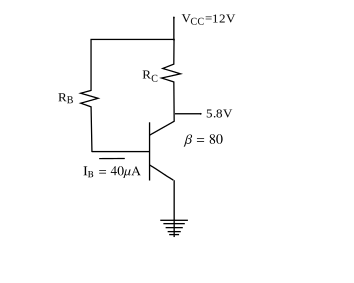
\includegraphics[scale=.95]{chap3/fig3.7.eps}
\end{figure}
\begin{align*}
\therefore\quad \rmI_{\rmC} &= \beta \rmI_{\rmB}=80\times 40\times 10^{-6}=3.2\text{~mA}\\[4pt]
\rmR_{\rmB} &= \frac{\rmV_{\text{CC}}-\rmV_{\text{BE}}}{\rmI_{\rmB}}=\dfrac{12-0.7}{40\times 10^{-6}}=282.5 \rmk\Omega\\[4pt]
\rmV_{\text{CE}} &= \rmV_{\rmC}=5.8\rmV.
\end{align*}
\begin{align*}
\text{We have}\qquad \rmV_{\text{CC}} &= \rmI_{\rmC}\rmR_{\rmC}+\rmV_{\text{CE}}\\[3pt]
\therefore\quad \rmR_{\rmC} &= \frac{\rmV_{\text{CC}}-\rmV_{\text{CE}}}{\rmI_{\rmC}}=\frac{12-5.8}{3.2\times 10^{-3}}=1.94\rmk\Omega.
\end{align*}
\end{solution}

\begin{problem}\label{prob3.2}
A transistor amplifier employing fixed bias circuit is subjected to an increase in temperature form $25^{\circ}$C to $75^{\circ}$C. If $\beta=100$ at $25^{\circ}$C and 150 at $75^{\circ}$C, determine the percentage change in Q-point values ($\rmI_{\rmC_{\rma}}$ and $\rmV_{\text{CE}_{\rmQ}}$ over the temperature range. Neglect the change in $\rmV_{\text{BE}}$ and leakage current $\rmI_{\text{CO}}$. Assume $\rmV_{\text{BE}}=0.7\rmV$. Given that $\rmV_{\text{CC}}=12\rmV$, $\rmR_{\rmB}=100\rmk\Omega$ and $\rmR_{\rmC}=560\Omega$.
\end{problem}

\begin{solution}
Given at $25^{\circ}$C : $\beta=100$ : $\rmV_{\text{CC}}=12\rmV$, \ $\rmR_{\rmB}=100\rmk$, \ $\rmR_{\rmC}=560\Omega$

at $75^{\circ}$C : $\beta=150$
\begin{align*}
\text{At}\quad 25^{\circ}\rmC\quad : \quad \rmI_{\rmC_{\rmQ}} &= \beta\left(\frac{\rmV_{\text{CC}}-\rmV_{\text{BE}}}{\rmR_{\rmB}}\right)=100\left(\frac{12-0.7}{100\times 10^{3}}\right)=11.3\text{~mA}\\[4pt]
\rmV_{\text{CE}_{\rmQ}} &= \rmV_{\text{CC}}-\rmI_{\rmC_{\rmQ}}\cdot \rmR_{\rmC}=12-(11.3\times 10^{-3})(560)=5.67\rmV\\[4pt]
\text{At}\quad 75^{\circ}\rmC\quad :\quad \rmI_{\rmC_{\rmQ}} &= \beta \left(\frac{\rmV_{\text{CC}}-\rmV_{\text{BE}}}{\rmR_{\rmB}}\right)=150\left(\frac{12-0.7}{100\times 10^{3}}\right)=16.95\text{~mA}\\[4pt]
\rmV_{\text{CE}_{\rmQ}} &= \rmV_{\text{CC}}-\rmI_{\rmC_{\rmQ}}\cdot \rmR_{\rmC} = 12-(16.95\times 10^{-3})(560)=2.5\rmV
\end{align*}
\begin{align*}
\therefore\quad \text{Percentage change in~~ $\rmI_{\rmC}$~ is } : \%\ \Delta \rmI_{\rmC} &= \frac{\rmI_{\rmC(75\%)}-\rmI_{\rmC(25^{\circ}\rmC)}}{\rmI_{\rmC(25^{\circ}\rmC)}}\times 100\%\\[4pt]
&= \frac{16.95\text{~mA}-11.3\text{~mA}}{11.3\text{~mA}}\times 100\%= 50\%\\[4pt]
\therefore\quad \text{Percentage change in~~ $\rmV_{\text{CE}}$~ is } : \%\ \Delta \rmV_{\text{CE}} &= \frac{\rmV_{\text{CE}(75^{\circ}\rmC)}-\rmV_{\text{CE}(25^{\circ}\rmC)}}{\rmV_{\text{CE}(25^{\circ}\rmC)}}\times 100\%\\[4pt]
&= \frac{2.5-5.67}{5.67}\times 100\% = -56\%
\end{align*}
\end{solution}

\begin{problem}\label{prob3.3}
For the fixed bias configuration shown, determine the Q-point. Also draw the dc load line. Assume $\rmV_{\text{BE}}$.
\begin{figure}[H]
\centering
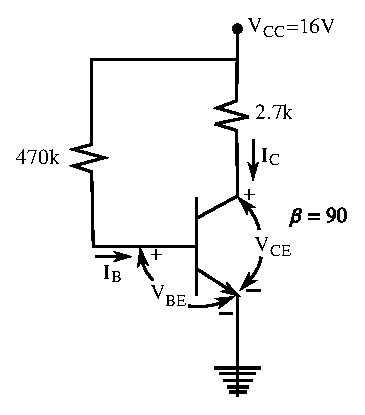
\includegraphics{chap3/fig3.8.eps}
\end{figure}
\end{problem}

\begin{solution}
\begin{align*}
\rmI_{\rmB_{\rmQ}} &= \frac{\rmV_{\text{CC}}-\rmV_{\text{BE}}}{\rmR_{\rmB}} = \frac{16-0.7}{470\times 10^{3}}=32.55\mu\rmA\\[4pt]
\rmI_{\rmC_{\rmQ}} &= \beta \rmI_{\rmB_{\rmQ}} = 90\times 32.55\times 10^{-6}=2.93\text{~mA}\\[4pt]
\rmV_{\text{CE}_{\rmQ}} &= \rmV_{\text{CC}}-\rmI_{\rmC_{\rmQ}}\cdot \rmR_{\rmC} = 16 - (2.93\times 10^{-3})(2.7\times 10^{3})
\end{align*}
The Q-point and dc load line are shown below.
\begin{figure}[H]
\centering
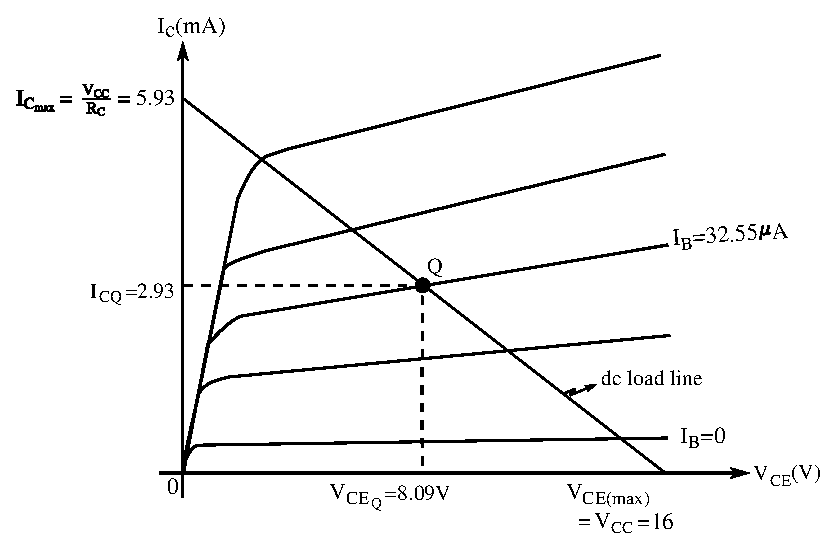
\includegraphics{chap3/fig3.9.eps}
\end{figure}
\end{solution}

\heading{Emitter-stabilized bias circuit~:} (Self bias circuit)

Fig. shows a transistor amplifier employing emitter - stabilized bias circuit. The contains an emitter resistor to improve the stability of Q-point.
\begin{figure}[H]
\centering
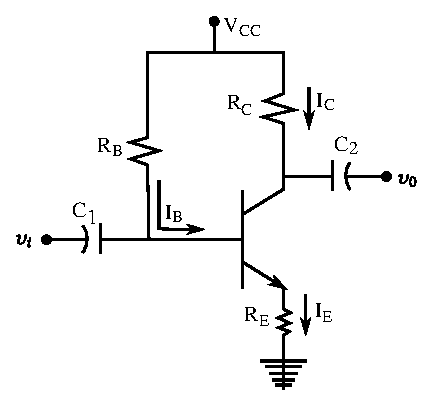
\includegraphics{chap3/fig3.10.eps}
\end{figure}

The dc equivalent circuit is shown below. A capacitors are replaced by open circuit.
\begin{figure}[H]
\centering
\includegraphics{chap3/fig3.11.eps}
\end{figure}

Applying KVL to the input side,
\begin{equation}
\rmV_{\text{CC}} = \rmI_{\rmB}\rmR_{\rmB}+\rmV_{\text{BE}}+\rmI_{\rmE}\rmR_{\rmE}\label{eq3.2}
\end{equation}
We have
\begin{equation}
\rmI_{\rmE}=\rmI_{\rmB}+\rmI_{\rmC}=\rmI_{\rmB}+\beta \rmI_{\rmB}=(\beta+1)\rmI_{\rmB}\label{eq3.3}
\end{equation}
Put Eqn.~\eqref{eq3.3} in Eqn.~\eqref{eq3.2}, 
\begin{align*}
\rmV_{\text{CC}} &= \rmI_{\rmB}\rmR_{\rmB}+\rmV_{\text{BE}}+(\beta+1)\rmI_{\rmB}\cdot \rmR_{\rmE}\\[4pt]
\therefore\quad \rmI_{\rmB} &= \frac{\rmV_{\text{CC}}-\rmV_{\text{BE}}}{\rmR_{\rmB}+(\beta+1)\rmR_{\rmE}}\quad\therefore\quad \rmI_{\rmC}=\beta \rmI_{\rmB}=\beta \left[\frac{\rmV_{\text{CC}}-\rmV_{\text{BE}}}{\rmR_{\rmB}+(\beta+1)\rmR_{\rmE}}\right]
\end{align*}
Applying KVL to the outside side,
\begin{align*}
\rmV_{\text{CC}} &= \rmI_{\rmC}\rmR_{\rmC}+\rmV_{\text{CE}}+\rmI_{\rmE}\rmR_{\rmE}\\[4pt]
\rmV_{\text{CC}} &= \rmI_{\rmC}(\rmR_{\rmC}+\rmR_{\rmE})+\rmV_{\text{CE}}\quad [\because \ \rmI_{\rmE}\simeq \rmI_{\rmC}]\\[4pt]
\therefore\quad \rmV_{\text{CE}} &= \rmV_{\text{CC}}-\rmI_{\rmC}(\rmR_{\rmC}+\rmR_{\rmE})\\[4pt]
\text{Also}\quad  \rmV_{\rmE}=\rmI_{\rmE}\rmR_{\rmE}; \ \rmV_{\rmB} &= \rmV_{\text{BE}}+\rmV_{\rmE}\quad\text{and}\quad \rmV_{\rmC}=\rmV_{\text{CE}}+\rmV_{\rmE}
\end{align*}

\eject

\begin{problem}\label{prob3.4}
For the emitter biased circuit shown, find 
\begin{itemize}
\item[(a)] $\rmI_{\rmB_{\rmQ}}$\quad (b)~ $\rmI_{\rmC_{\rmQ}}$\quad (c)~ $\rmV_{\text{CE}_{\rmQ}}$\quad (d)~ $\rmV_{\rmC}$\quad (e)~ $\rmV_{\rmB}$ and $\rmV_{\rmE}$.
\end{itemize}
Assume $\rmV_{\text{BE}}=0.7\rmV$.
\begin{figure}[H]
\centering
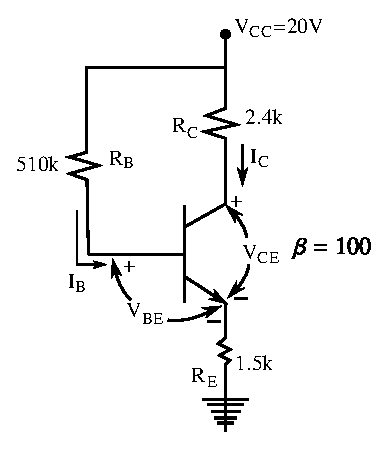
\includegraphics{chap3/fig3.12.eps}
\end{figure}
\end{problem}

\begin{solution}
\begin{itemize}
\item[(a)] $\rmI_{\rmB_{\rmQ}}=\dfrac{\rmV_{\text{CC}}-\rmV_{\text{BE}}}{\rmR_{\rmB}+(\beta+1)\rmR_{\rmE}}=\dfrac{20-0.7}{510\times 10^{3}+101\times 1.5\times 10^{3}}=29.18\mu\rmA$

\item[(b)] $\rmI_{\rmC_{\rmQ}}=\beta \rmI_{\rmB_{\rmQ}}=100\times 29.18\times 10^{-6}=2.91\text{~mA}$

\item[(c)] 
\begin{tabbing}
$\rmV_{\text{CE}_{\rmQ}}=\rmV_{\text{CC}}-\rmI_{\rmC}(\rmR_{\rmC}+\rmR_{\rmE})$ \== $20-2.91\times 10^{-3}(2.4\times 10^{3}+1.5\times ????)$\\[4pt]
\>= 8.65\,V
\end{tabbing}

$\rmI_{\rmE_{\rmQ}}=\rmI_{\rmB}+\rmI_{\rmC}=29.18\times 10^{-6}+2.91\times 10^{-3}=2.94\text{~mA}$

\item[(c)] $\rmV_{\rmC}=\rmV_{\text{CE}}+\rmI_{\rmE}\rmR_{\rmE}=8.65+2.94\times 10^{-3}\times 1.5\times 10^{3}=13.06\rmV$

\item[(e)]
\begin{tabbing}
$\rmV_{\rmE}$ \== $\rmI_{\rmE}\rmR_{\rmE}=2.94\times 10^{-3}\times 1.5\times 10^{3}=4.41\rmV$\\[4pt]
$\rmV_{\rmB}$ \>= $\rmV_{\text{BE}}+\rmV_{\rmE}=0.7+4.41=5.11\rmV$
\end{tabbing}
\end{itemize}
\end{solution}

\eject

\begin{problem}\label{prob3.5}
For the emitter biased circuit shown, find
\begin{itemize}
\item[(a)] $\rmR_{\rmC}$\quad (b)~ $\rmR_{\rmE}$\quad (c)~ $\rmR_{\rmB}$\quad (d)~ $\rmV_{\text{CE}}$~~ and~~ (e)~ $\rmV_{\rmB}$
\end{itemize}
\noindent
\begin{minipage}[c]{7cm}
\begin{figure}[H]
\centering
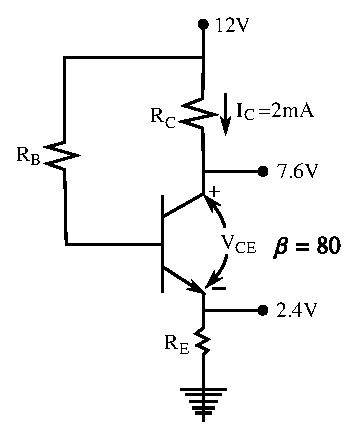
\includegraphics{chap3/fig3.13.eps}
\end{figure}
\end{minipage}
\qquad
\begin{minipage}[c]{7cm}
\begin{align*}
\text{Given~:}\qquad \rmV_{\text{CC}} &= 12\rmV\\[3pt]
\rmI_{\rmC} &= 2\text{~mA}\\[3pt]
\rmV_{\rmC} &= 7.6\rmV\\[3pt]
\rmV_{\rmE} &= 2.4\rmV\\[3pt]
\beta &= 80
\end{align*}
\end{minipage}
\end{problem}

\begin{solution}
\begin{align*}
\rmI_{\rmB_{\rmQ}} &= \frac{\rmI_{\rmC_{\rmQ}}}{\beta}=\dfrac{2\times 10^{-3}}{80}=25\mu\rmA\\[4pt]
\rmV_{\text{CE}_{\rmQ}} &= \rmV_{\rmC}-\rmV_{\rmE}=7.6-2.4=5.2\rmV\\[4pt]
\rmI_{\rmE_{\rmQ}} &= \rmI_{\rmB}+\rmI_{\rmC}=25\times 10^{-6}+2\times 10^{-3}=2.025\text{~mA}\\[4pt]
\therefore\quad \rmV_{\rmE} &= \rmI_{\rmE}\rmR_{\rmE}\Rightarrow \rmR_{\rmE}=\dfrac{\rmV_{\rmE}}{\rmI_{\rmE}}=\dfrac{2.4}{2.025\times 10^{-3}}=1.185\rmk\Omega\\[4pt]
\rmV_{\rmB} &= \rmV_{\rmB\rmE}+\rmV_{\rmE}=0.7+2.4=3.1\rmV\\[4pt]
\rmR_{\rmC} &= \frac{\rmV_{\text{CC}}-\rmV_{\rmC}}{\rmI_{\rmC}}=\frac{12-7.6}{2\times 10^{-3}}=2.2\rmk\Omega\\[4pt]
\rmR_{\rmB} &= \frac{\rmV_{\text{CC}}-\rmV_{\rmB}}{\rmI_{\rmB}}=\frac{12-3.1}{25\times 10^{-6}}=356\rmk\Omega
\end{align*}
\end{solution}

\begin{problem}\label{prob3.6}
A transistor amplifier employing emitter stabilized bias circuit is subjected to an increase in temperature from $25^{\circ}$C to $75^{\circ}$C. If $\beta=100$ at $25^{\circ}$C and 150 at $75^{\circ}$C, determine the percentage change, Q-point values ($\rmI_{\rmC_{\rmQ}}$ and $\rmV_{\text{CE}_{\rmQ}}$) over the temperature range. Neglect be change in $\rmV_{\text{BE}}$ and leakage current $\rmI_{\text{CO}}$. Assume $\rmV_{\text{BE}}=0.7\rmV$. Given that $\rmV_{\text{CC}}=20\rmV$, $\rmR_{\rmB}=510\rmk\Omega$, $\rmR_{\rmC}=2.4\rmk\Omega$ and $\rmR_{\rmE}=1.5\rmk\Omega$.  
\end{problem}

\begin{solution}
Given that at $25^{\circ}$C : $\beta=100$; at $75^{\circ}C$ : $\beta=150$.
\begin{align*}
\text{At~}25^{\circ}\rmC~ :~ \rmI_{\rmC_{\rmQ}} &=\beta\left(\frac{\rmV_{\text{CC}}-\rmV_{\text{BE}}}{\rmR_{\rmB}+(\beta+1)\rmR_{\rmE}}\right)=100\left(\frac{20-0.7}{510\times 10^{3}+(101)(1.5\times 10^{3})}\right)=2.91\text{~mA}\\[4pt]
\rmV_{\text{CE}_{\rmQ}} &= \rmV_{\text{CC}}-\rmI_{\rmC_{\rmQ}}(\rmR_{\rmC}+\rmR_{\rmE})=20-2.91\times 10^{-3}(2.4\times 10^{3}+1.5\times 10^{3})=8.65\rmV\\[4pt]
\text{At~} 75^{\circ}\rmC~ :~ \rmI_{\rmC_{\rmQ}} &= \beta \rmI_{\rmB_{\rmQ}}=\beta \left(\frac{\rmV_{\text{CC}}-\rmV_{\text{BE}}}{\rm_{\rmB}+(\beta+1)\rmR_{\rmE}}\right)=150 \left(\frac{20-0.7}{510\times 10^{3}+(151)(1.5\times 10^{3})}\right)=3.93\text{~mA}\\[4pt]
\rmV_{\text{CE}_{\rmQ}} &= \rmV_{\text{CC}}-\rmI_{\rmC_{\rmQ}}(\rmR_{\rmC}+\rmR_{\rmE})=20-3.93\times 10^{-3}(2.4\times 10^{3}+1.5\times 10^{3})=4.67\rmV
\end{align*}
\begin{align*}
\text{Percentage change in~} \rmI_{\rmC} : \ \%\ \Delta \rmI_{\rmC} &= \frac{\rmI_{\rmC(75^{\circ}\rmC)}-\rmI_{\rmC(25^{\circ}\rmC)}}{\rmI_{\rmC(25^{\circ}\rmC)}}\times 100\%\\[4pt]
&= \frac{3.93-2.91}{2.91}\times 100\% = 35.1\%\\[4pt]
\text{Percentage change in~} \rmV_{\text{CE}} : \%\ \Delta \rmV_{\text{CE}} &= \frac{\rmV_{\text{CE}(75^{\circ}\rmC)}-\rmV_{\text{CE}(25^{\circ}\rmC)}}{\rmV_{\text{CE}(25^{\circ}\rmC)}}\times 100\%\\[4pt]
&= \frac{4.67-8.65}{8.65}\times 100\% = -46.01\%
\end{align*}

Fig. shows a transistor amplifier employing collector - base feedback bias circuit. It provides more stability of Q-point compared to fixed and emitter stabilized bias circuit.
\begin{figure}[H]
\centering
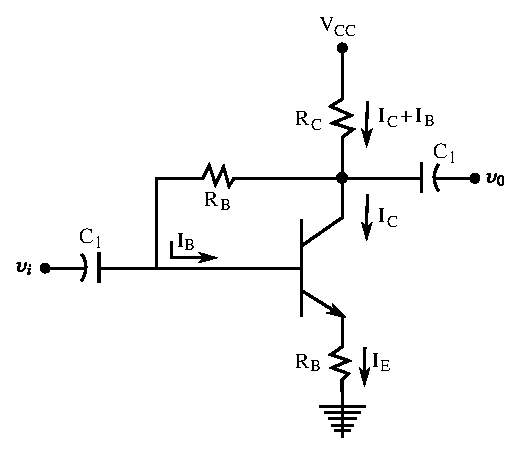
\includegraphics{chap3/fig3.14.eps}
\end{figure}

The dc equivalent circuit is shown below.
\begin{figure}[H]
\centering
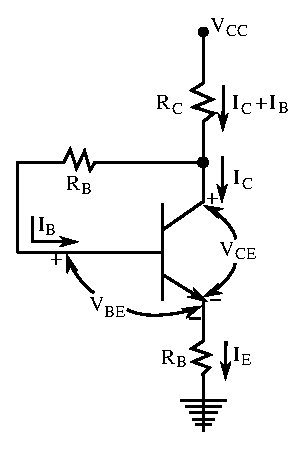
\includegraphics{chap3/fig3.15.eps}
\end{figure}

Applying KVL to the input side,
\begin{align*}
& \rmV_{\text{CC}}-(\rmI_{\rmC}+\rmI_{\rmB})\rmR_{\rmC}-\rmI_{\rmB}\rmR_{\rmB}-\rmV_{\text{BE}}-\rmI_{\rmE}\rmR_{\rmE}=0\\[4pt]
& \rmV_{\text{CC}}-(\beta+1)\rmI_{\rmB}\rmR_{\rmC}+\rmI_{\rmB}\rmR_{\rmB}+\rmV_{\text{BE}}+(\beta+1)\rmI_{\rmB}\rmR_{\rmE}
\end{align*}
\begin{align*}
\therefore\quad \rmI_{\rmB} &= \frac{\rmV_{\text{CC}}-\rmV_{\text{BE}}}{\rmR_{\rmB}+(\beta+1)(\rmR_{\rmC}+\rmR_{\rmE})}\\[4pt]
\rmI_{\rmC} &= \beta \rmI_{\rmB}=\beta\left[\frac{\rmV_{\text{CC}}-\rmV_{\text{BE}}}{\rmR_{\rmB}+(\beta+1)(\rmR_{\rmC}+\rmR_{\rmE})}\right]
\end{align*}
Applying KVL to the output side,
\begin{align*}
\rmV_{\text{CC}} &= (\rmI_{\rmC}+\rmI_{\rmB})\rmR_{\rmC}+\rmV_{\text{CE}}+\rmI_{\rmE}\rmR_{\rmE}\\[4pt]
&= \rmI_{\rmE}\rmR_{\rmC}+\rmV_{\text{CE}}+\rmI_{\rmE}\rmR_{\rmE}=\rmI_{\rmE}(\rmR_{\rmC}+\rmR_{\rmE})+\rmV_{\text{CE}}\simeq \rmI_{\rmC}(\rmR_{\rmC}+\rmR_{\rmE})+\rmV_{\text{CE}}\\[4pt]
\therefore\quad \rmV_{\text{CE}} &= \rmV_{\text{CC}}-\rmI_{\rmC}(\rmR_{\rmC}+\rmR_{\rmE})
\end{align*}
\end{solution}

\begin{problem}\label{prob3.7}
For the collector-base feedback bias circuit shows determine
\begin{itemize}
\item[(a)] $\rmI_{\rmC}$\quad (b)~ $\rmV_{\rmC}$\quad (c)~ $\rmV_{\rmE}$\quad and\quad (d)~ $\rmV_{\text{CE}}$.
\end{itemize}
Assume $\rmV_{\text{BE}}=0$?????
\begin{figure}[H]
\centering
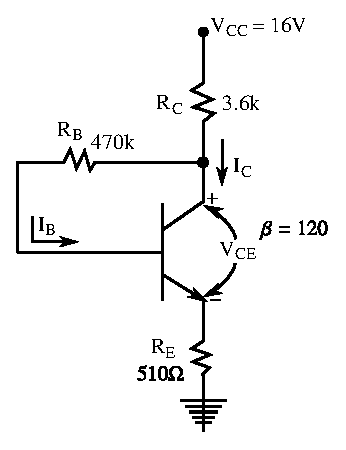
\includegraphics[scale=.87]{chap3/fig3.16.eps}
\end{figure}
\end{problem}

\begin{solution}
\begin{align*}
\rmI_{\rmB_{\rmQ}} &= \frac{\rmV_{\text{CC}}-\rmV_{\text{BE}}}{\rmR_{\rmB}+(\beta+1)(\rmR_{\rmC}+\rmR_{\rmE})}=\frac{16-0.7}{470\times 10^{3}+(121)(3.6\times 10^{3}+510)}=15.8\\[4pt]
\therefore\quad \rmI_{\rmC_{\rmQ}} &= \beta \rmI_{\rmB_{\rmQ}}=120\times 15.8\times 10^{-6}=1.9\text{~mA}\\[4pt]
\rmV_{\text{CE}} &= \rmV_{\text{CC}}-\rmI_{\rmC}(\rmR_{\rmC}+\rmR_{\rmE})=16-1.9\times 10^{-3}[3.6\times 10^{3}+510]=8.21\\[4pt]
\rmV_{\rmE} &= \rmI_{\rmE}\rmR_{\rmE}=(\rmI_{\rmB}+\rmI_{\rmC})\rmR_{\rmE}=(15.8\times 10^{-6}+1.9\times 10^{-3})510=0.98\rmV\\[4pt]
\rmV_{\rmC} &= \rmV_{\text{CE}}+\rmV_{\rmE}=8.2+0.98=9.18\rmV
\end{align*}
\end{solution}

\begin{problem}\label{prob3.8}
Determine the range of possible values of $\rmV_{\rmC}$ for the circuit shown below using the $1\rmM\Omega$ potentiometer.

\noindent
\begin{minipage}[c]{7cm}
\begin{figure}[H]
\centering
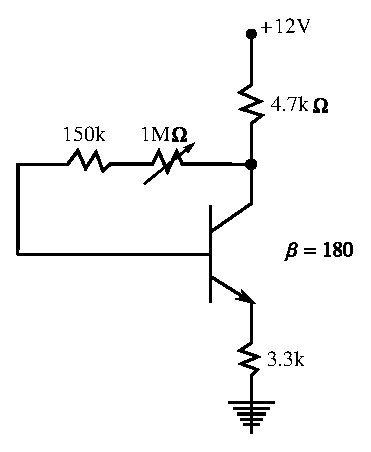
\includegraphics[scale=.87]{chap3/fig3.17.eps}
\end{figure}
\end{minipage}
\quad
\begin{minipage}[c]{7cm}
\begin{align*}
\text{Given~:}\qquad \rmV_{\text{CC}} &= +12\rmV\\[3pt]
\beta &= 180\\[3pt]
\rmR_{\rmC} &= 4.7\rmk\Omega\\[3pt]
\rmR_{\rmE} &= 3.3\rmk\Omega
\end{align*}
\end{minipage}
\end{problem}

\begin{solution}
When $\rmR_{\rmB}$ is minimum, $\rmR_{\rmB}=150\rmk\Omega+0=150\rmk\Omega$.
\begin{align*}
\rmI_{\rmB_{\rmQ}} &= \frac{\rmV_{\text{CC}}-\rmV_{\text{BE}}}{\rmR_{\rmB}+(\beta+1)(\rmR_{\rmC}+\rmR_{\rmE})}=\dfrac{12-0.7}{150\times 10^{3}+(181)(4.7\times 10^{3}+3.3\times 10^{3})}=7.1\\[3pt]
\rmI_{\rmC_{\rmQ}} &= \beta \rmI_{\rmB_{\rmQ}}=180\times 7.7\times 10^{-6}=1.27\text{~mA}\\[3pt]
??? &= ????????????????????\\[3pt]
??? &= ????????????????????\\[3pt]
\therefore\quad \rmV_{\rmC} &= \rmV_{\text{CE}} +\rmV_{\rmE}=\rmV_{\text{CE}}+\rmI_{\rmE}\rmR_{\rmE}=1.84+(1.28\times 10^{-3}\times 3.3\times 10^{3})=6.06\rmV
\end{align*}
When $\rmR_{\rmB}$ is maximum, $\rmR_{\rmB}=150\rmk\Omega+1\rmM\Omega=1.15\rmM\Omega$.
\begin{align*}
\rmI_{\rmB_{\rmQ}} &= \frac{\rmV_{\text{CC}}-\rmV_{\text{BE}}}{\rmR_{\rmB}+(\beta+1)(\rmR_{\rmC}+\rmR_{\rmE})}=\frac{12-0.7}{1.15\times 10^{6}+(181)(4.7\times 10^{3}+3.3\times 10^{3})}=4.35\mu\rmA\\[3pt]
\rmI_{\rmC_{\rmQ}} &= \beta \rmI_{\rmB_{\rmQ}} = 180\times 4.35\times 10^{-6}=0.783\text{~mA}\\[3pt]
\rmI_{\rmE_{\rmQ}} &= \rmI_{\rmB}+\rmI_{\rmC}=4.35\mu+0.783\rmm=0.787\text{~mA}\\[3pt]
\rmV_{\text{CE}_{\rmQ}} &= \rmV_{\text{CC}}-\rmI_{\rmC}(\rmR_{\rmC}+\rmR_{\rmE})=12-0.783\times 10^{-3}(4.7\times 10^{3}+3.3\times 10^{3})=5.736\rmV\\[3pt]
\therefore\quad \rmV_{\rmC} &= \rmV_{\text{CE}}+\rmV_{\rmE}=\rmV_{\text{CE}}+\rmI_{\rmE}\rmR_{\rmE}=5.736+(0.787\rmm)(3.3\rmk)=8.33\rmV.
\end{align*}
$\therefore$~~ $\rmV_{\rmC}$ ranges from $6.06\rmV$ to $8.33\rmV$.
\end{solution}

\begin{problem}\label{prob3.9}
For the network shown, determine
\begin{itemize}
\item[(a)] $\rmI_{\rmC}$\quad (b)~ $\rmV_{\rmC}$\quad (c)~ $\rmV_{\rmE}$ \ \ and \ \ (d)~ $\rmV_{\text{CE}}$
\end{itemize}
\begin{figure}[H]
\centering
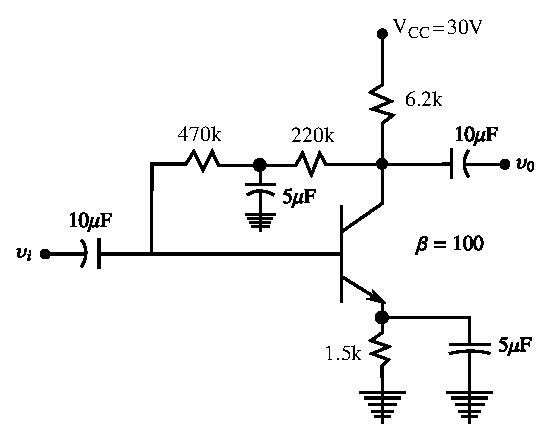
\includegraphics[scale=.9]{chap3/fig3.18.eps}
\end{figure}
\end{problem}

\begin{solution}
Writing the dc equivalent circuit (replace all capacitors by open circuit).

\noindent
\begin{minipage}[c]{7cm}
\begin{figure}[H]
\centering
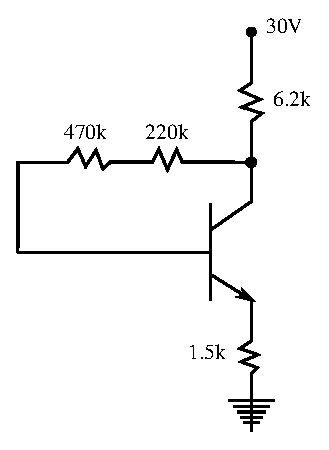
\includegraphics[scale=.9]{chap3/fig3.19.eps}
\end{figure}
\end{minipage}
\quad
\begin{minipage}[c]{7cm}
\begin{align*}
\text{Given~:}\qquad \rmV_{\text{CC}} &= 30\rmV\\[3pt]
\beta &= 100\\[3pt]
\rmR_{\rmC} &= 6.2\rmk\Omega\\[3pt]
\rmR_{\rmE} &= 1.5\rmk\Omega\\[3pt]
\rmR_{\rmB} &= 470\rmK+220\rmK=690\rmK
\end{align*}
\end{minipage}
\begin{align*}
\rmI_{\rmB} &= \frac{\rmV_{\text{CC}}-\rmV_{\text{BE}}}{\rmR_{\rmB}+(\beta+1)(\rmR_{\rmC}+\rmR_{\rmE})}\\[5pt]
&=\dfrac{30-0.7}{690\rmK+(101)(6.2\rmK+1.5\rmK)}=20\\[5pt]
\therefore\quad \rmI_{\rmC} &= \beta \rmI_{\rmB}=100\times 20\mu = 2\text{~mA}\\[5pt]
\rmV_{\text{CE}} &= \rmV_{\text{CC}}-\rmI_{\rmC}(\rmR_{\rmC}+\rmR_{\rmE})\\[5pt]
&= 30-(2\rm)(6.2\rmK+1.5\rmK)\\[5pt]
&= 14.6\rmV\\[5pt]
\rmI_{\rmE} &= \rmI_{\rmB}+\rmI_{\rmC}=20\mu+2\text{~mA}=2.02\text{~mA}\\[5pt]
\rmV_{\rmC} &= \rmV_{\text{CE}}+\rmI_{\rmE}\rmR_{\rmE}\\[5pt]
&= 14.63+(2.02\rm)(1.5\rmK)\\[5pt]
&= 17.66\rmV\\[5pt]
\rmV_{\rmE} &= \rmI_{\rmE}\rmR_{\rmE}=(2.02\rmm)(1.5\rmk)\\[5pt]
&\quad 3.03\rmV
\end{align*}
\end{solution}

\eject

\heading{(iv)~ Voltage divider bias circuit~:}
\begin{figure}[H]
\centering
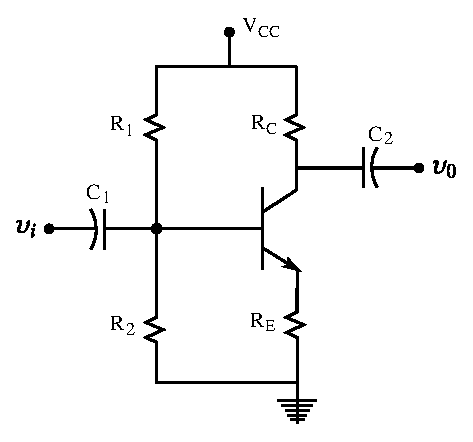
\includegraphics{chap3/fig3.20.eps}
\end{figure}

Fig. shows a transistor amplifier employing voltage divider bias circuit. It is also called universal bias circuit. The dc equivalent circuit is shown below.
\begin{figure}[H]
\centering
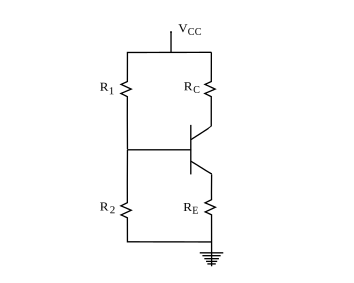
\includegraphics{chap3/fig3.21.eps}
\end{figure}

\eject

Replacing the input side with its Thevinin equivalent circuit the above circuit can be written as,
\begin{figure}[H]
\centering
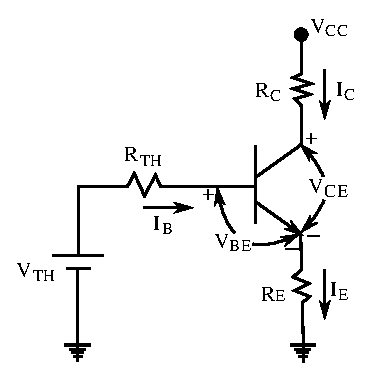
\includegraphics{chap3/fig3.22.eps}
\end{figure}
\begin{align*}
\rmV_{\text{TH}} &= \frac{\rmV_{\text{CC}}\cdot \rmR_{2}}{\rmR_{1}+\rmR_{2}}\\[4pt]
\rmR_{\text{TH}} &= \rmR_{1} || \rmR_{2}=\frac{\rmR_{1}\rmR_{2}}{\rmR_{1}+\rmR_{2}}
\end{align*}

Applying KVL to input side,
\begin{align*}
& \rmV_{\text{TH}} - \rmI_{\rmB}\rmR_{\text{TH}}-\rmV_{\text{BE}}-\rmI_{\rmE}\rmR_{\rmE}=0\\[3pt]
& \rmV_{\text{TH}} = \rmI_{\rmB}\rmR_{\text{TH}}+\rmV_{\text{BE}}+(\beta+1)\rmI_{\rmB}\rmR_{\rmE}\\[3pt]
\therefore\quad & \rmI_{\rmB} = \frac{\rmV_{\text{TH}}-\rmV_{\text{BE}}}{\rmR_{\text{TH}}+(\beta+1)\rmR_{\rmE}}\\[3pt]
\therefore\quad & \rmI_{\rmC} = \beta \rmI_{\rmB}=\beta\left[\frac{\rmV_{\text{TH}}-\rmV_{\text{BE}}}{\rmR_{\text{TH}}+(\beta+1)\rmR_{\rmE}}\right]
\end{align*}
Applying KVL to the output side,
\begin{align*}
& \rmV_{\text{CC}}-\rmI_{\rmC}\rmR_{\rmC}-\rmV_{\text{CE}}-\rmI_{\rmE}\rmR_{\rmE}=0\\[3pt]
& \rmV_{\text{CC}}=\rmI_{\rmC}(\rmR_{\rmC}+\rmR_{\rmE})+\rmV_{\text{CE}}\quad [\because ~~ \rmI_{\rmE}\simeq \rmI_{\rmC}]\\[3pt]
\therefore\quad & \rmV_{\text{CE}}=\rmV_{\text{CC}}-\rmI_{\rmC}(\rmR_{\rmC}+\rmR_{\rmE})
\end{align*}

\eject

\begin{problem}\label{prob3.10}
Int he circuit shown, determine 
\begin{itemize}
\item[(a)] $\rmI_{\rmB_{\rmQ}}$\quad (b)~ $\rmI_{\rmC_{\rmQ}}$\quad (c)~ $\rmV_{\text{CE}_{\rmQ}}$\quad (d)~ $\rmV_{\rmC}$\quad (e)~ $\rmV_{\rmE}$\quad (f)~ $\rmV_{\rmB}$\quad (g)~ $\rmI_{\rmC(\text{sat})}$.
\end{itemize}
Also draw dc load line.
\begin{figure}[H]
\centering
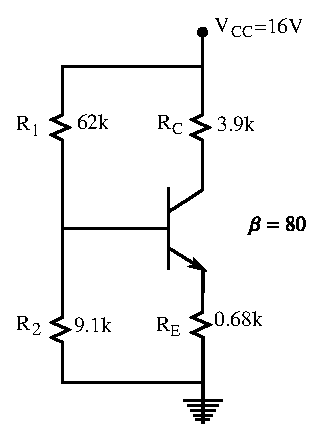
\includegraphics{chap3/fig3.23.eps}
\end{figure}
\end{problem}

\begin{solution}
Writing Thevinins equivalent on input side,

\noindent
\begin{minipage}[c]{7cm}
\begin{figure}[H]
\centering
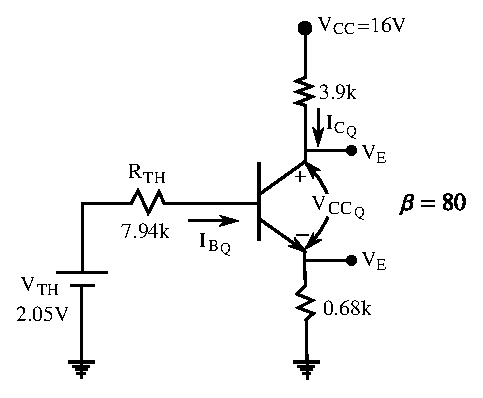
\includegraphics{chap3/fig3.24.eps}
\end{figure}
\end{minipage}
\quad
\begin{minipage}[c]{7cm}
\begin{align*}
\rmV_{\text{TH}} &= \frac{\rmV_{\text{CC}}\rmR_{2}}{\rmR_{1}+\rmR_{2}}=\frac{16\times 19.1\rmK}{62\rmK+9.1}\\[4pt]
\rmR_{\text{TH}} &= \rmR_{1}||\rmR_{2} = \frac{\rmR_{1}\rmR_{2}}{\rmR_{1}+\rmR_{2}}=\frac{62\rmK}{62\rmK}\\[4pt]
&= 7.94\rmK\Omega.
\end{align*}
\end{minipage}
\smallskip
\begin{align*}
\rmI_{\rmB_{\rmQ}} &= \frac{\rmV_{\text{TH}}-\rmV_{\text{BE}}}{\rmR_{\text{TH}}+(\beta+1)\rmR_{\rmE}}=\frac{2.05-0.1}{7.94\rmK+(81)(0.68\rmK)}=21.42\mu \rmA\\[3pt]
\rmI_{\rmC_{\rmQ}} &= \beta \rmI_{\rmB_{\rmQ}}=80\times 21.42\mu=1.71\text{~mA}\\[3pt]
\rmV_{\text{CE}_{\rmQ}} &= \rmV_{\text{CC}}-\rmI_{\rmC}(\rmR_{\rmC}+\rmR_{\rmE})=16-(1.71\rmm)(3.9\rmK+0.68\rmK)=8.17\rmV\\[3pt]
\rmV_{\rmE} &= \rmI_{\rmE}\rmR_{\rmE}\simeq \rmI_{\rmC}\rmR_{\rmE}=(1.71\rmm)(0.68\rmK)=1.16\rmV\\[3pt]
\rmV_{\rmC} &= \rmV_{\text{CE}}+\rmV_{\rmE}=8.17+1.16=9.33\rmV\\[3pt]
\rmV_{\rmB} &= \rmV_{\text{BE}}+\rmV_{\rmE}=0.7+1.16=1.86\rmV
\end{align*}
Applying KVL to the output side,
\begin{align}
\rmV_{\text{CC}} &= \rmI_{\rmC}\rmR_{\rmC}+\rmV_{\text{CE}}+\rmI_{\rmE}\rmR_{\rmE}\notag\\[3pt]
&= \rmV_{\text{CE}}+\rmI_{\rmC}(\rmR_{\rmC}+\rmR_{\rmE})\quad [\because \ \rmI_{\rmC}\simeq \rmI_{\rmE}]\label{eq3.4}
\end{align}
Eqn.~\eqref{eq3.4}, When $\rmV_{\text{CE}}=0$
$$
\rmI_{\rmC}=\rmI_{\text{sat}}=\frac{\rmV_{\text{CC}}}{\rmR_{\rmC}+\rmR_{\rmE}}=\frac{16}{3.9\rmK+0.68\rmK}=3.49\text{~mA}
$$
When $\rmI_{\rmC}=0$
$$
\rmV_{\text{CE}}=\rmV_{\text{CE}_{\max}}=\rmV_{\text{CC}}=16\rmV
$$
\begin{figure}[H]
\centering
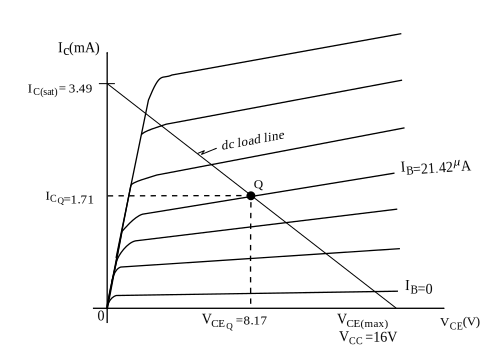
\includegraphics[scale=.9]{chap3/fig3.25.eps}
\end{figure}
\end{solution}

\eject

\begin{problem}\label{prob3.11}
In the circuit shown below, find $\rmI_{\rmC}$, $\rmV_{\rmE}$, $\rmV_{\rmB}$ and $\rmR$????
\begin{figure}[H]
\centering
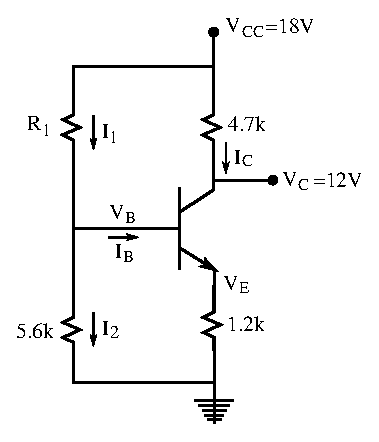
\includegraphics{chap3/fig3.26.eps}
\end{figure}
\end{problem}

\begin{solution}
\begin{align*}
\rmI_{\rmC} &= \frac{\rmV_{\text{CC}}-\rmV_{\rmC}}{\rmR_{\rmC}} = \frac{18-12}{4.7\rmK}=1.28\text{~mA}\\[3pt]
\therefore\quad \rmV_{\rmE} &= \rmI_{\rmE}\rmR_{\rmE}\simeq \rmI_{\rmC}\rmR_{\rmE}=(1.28\rmm)(1.2\rmK)=1.54\rmV\quad [\because \ \ \rmI_{\rmE}\simeq \rmI_{\rmC}]\\[3pt]
\therefore\quad \rmV_{\text{CE}} &= \rmV_{\rmC}-\rmV_{\rmE}=12-1.54=10.46\rmV\\[3pt]
\rmV_{\rmB} &= \rmV_{\text{BE}}+\rmV_{\rmE}=0.7+1.54=2.24\rmV
\end{align*}
In the circuit
\begin{align*}
\rmI_{2} &= \frac{\rmV_{\rmB}}{5.6\rmK}=\frac{2.24}{5.6\rmK}=400\mu\rmA\\[3pt]
\text{Also}\quad \rmI_{1} &= \rmI_{\rmB}+\rmI_{2}\\[3pt]
\rmI_{1} &\simeq \rmI_{2}\quad [\because \ \rmI_{\rmB}\text{~~ is very small}]\\[3pt]
\therefore\quad \rmI_{1} &\simeq \rmI_{2} =\frac{\rmV_{\text{CC}}-\rmV_{\rmB}}{\rmR_{1}}=400\mu\rmA\\[3pt]
\therefore\quad \rmR_{1} &= \frac{\rmV_{\text{CC}}-\rmV_{\rmB}}{400\mu}\\[3pt]
&= \frac{18-2.24}{400\mu}=39.4\rmK\Omega
\end{align*}
\end{solution}


\label{3end}
